\section{Introduzione}
\diapo{Le diossine}\pause
Tra i circa duecento derivati stabili della 1,4-diossina i più noti sono le dibenzodiossine policlorurate o PCDD (\emph{Polychlorinated dibenzodioxins}).
\begin{columns}
\column{0.3\linewidth}\begin{figure}{\centering{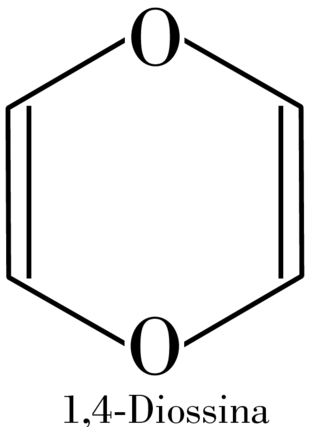
\includegraphics[width=0.3\textwidth]{img/1,4.png}}}\end{figure}
\column{0.7\linewidth}\begin{figure}{\centering{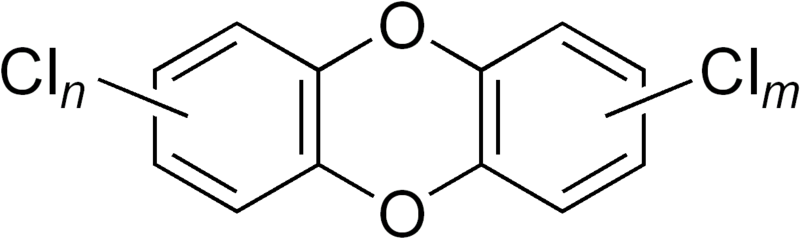
\includegraphics[width=0.5\textwidth]{img/diossine.png}}}\end{figure}
\end{columns}
Gergalmente col  {\bf termine ``diossina'' si intende  l'intera classe delle diossine e diossino simili, furani, diossani e PCB coplanari compresi}.
\pause

In questa ricerca si tratteranno  {\bf solo metodi di analisi per diossine propriamente dette} o dibenzodiossine policlorurate.
\end{frame}


\diapo{Formazione delle diossine}
Le diossine vengono prodotte se sussistono le seguenti condizioni:

\begin{itemize}
  \item presenza di  {\bf sostanze organiche clorurate};
  \item presenza di  {\bf metalli} di transizione;
   \item presenza di  materiali organici attaccabili dal cloro;
   \item  {\bf temperature} comprese tra 200 e 500 °C;
 \item combustione in presenza di  {\bf ossigeno in difetto};
  \item assenza di zolfo.
\end{itemize}
Si possono verificare facilmente in  {\bf inceneritori urbani e fonderie}.
\end{frame}
\begin{frame}\frametitle{Formazione delle diossine}
Le emissioni più importanti avvengono, in ordine di flusso:
\begin{enumerate}
\item nel terreno: causa i {\bf  pesticidi }(sia in fase di produzione che di uso), i {\bf  fuochi} accidentali e lo smaltimento dei  {\bf rifiuti};
\item nell'atmosfera: causa  {\bf l'incenerimento dei rifiuti} e il settore industriale  {\bf siderurgico};
\item nelle acque: dilavamento dal terreno, settore chimico, discariche di rifiuti, produzione di carta, incenerimento e smaltimento degli olii usati.
\end{enumerate}
\end{frame}


\diapo{Tossicità delle diossine}
Tra le diossine si conoscono 17 composti tossici. L'isomero annoverato tra i più potenti veleni conosciuti è la {\bf 2,3,7,8-tetraclorodibenzo-p-diossina} anche detta impropriamente TCDD.
\pause

Il suo LD50 per via orale nella cavia è di 500 ng/kg. La tossicità degli altri isomeri è riferita come   {\bf fattore di equivalenza tossica (TEF)} ossia un rapporto tra concentrazioni a parità di effetto tossico con la TCDD. 

La   {\bf tossicità equivalente (TEQ)} in un campione è una somma delle masse pesate per il fattore TEF.
\pause

L'effetto tossico delle diossine deriva dall'interazione col recettore cellulare AHR aryl hydrocarbon receptor, un fattore trascrizionale genico.
\begin{figure}{\centering{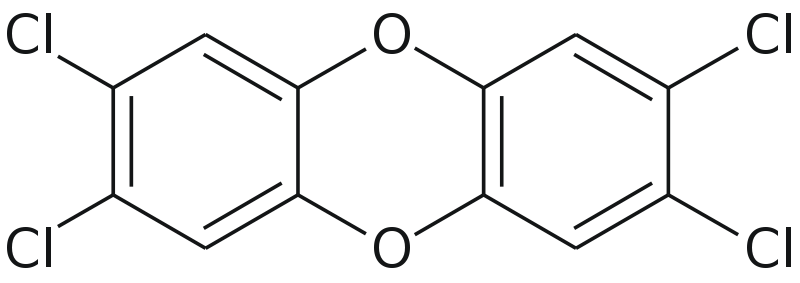
\includegraphics[width=0.35\textwidth]{img/tcdd.png}}}\end{figure}


\end{frame}

\diapo{Perché analizzare le diossine nel terreno?}
Le diossine hanno un tempo di emivita in esseri viventi di alcuni anni e sono molto lipofile. Per questi motivi danno il fenomeno di   {\bf bioaccumulazione}.


  {\bf Il principale meccanismo con cui le diossine entrano nella catena alimentare terrestre è tramite le piante coltivate in terreni inquinati}.
\pause

La contaminazione di queste piante segue meccanismi di assorbimento di vapori e di deposizione sulle foglie di particolato secco che supporta diossine. 

È perciò importante valutarne la concentrazione nel suolo.


\end{frame}


\diapo{Panoramica delle metodologie analitiche}
L'elevatissima tossicità porta alla   {\bf necessità di sensibilità piuttosto elevate} per rivelare quantità dell'ordine dei picogrammi.
\pause

Le procedure analitiche seguono grossomodo il seguente schema: 
\begin{enumerate}
 \item   {\bf estrazione} di diossine dal campione di terreno (Soxhlet, ASE, PLE, sistemi micellari e microonde, \ce{CO2} supercritica, ultrasuoni e SPME dello spazio di testa),
 \item   {\bf lavaggio e concentrazione} (trappole di carbone attivo o allumina attivata, essiccamento con centrifuga a vuoto),
 \item   {\bf separazione} degli analiti di interesse dagli interferenti (colonne in serie, HPLC),
 \item   {\bf rivelazione tramite} cattura elettronica, saggi di tossicità o ionizzazione ed analisi con spettrometria di massa.
\end{enumerate}
\end{frame}



\subsection{I metodi}\subsubsection{Il metodo di riferimento}\begin{frame}\frametitle{I metodi}\framesubtitle{Il metodo di riferimento}
Il {\bf metodo di riferimento} per l'analisi delle diossine è stato redatto nel 2005 dalla  {\bf  Japanese Industrial Standard}\footnote{J. Standard Association, JIS K0311, 2005. Documento a pagamento.} ed impiega:
\begin{itemize}
 \item HRGC \emph{high resolution gas chromatography},
 \item ionizzazione con \emph{electron beam},
 \item HRMS \emph{high resolution mass sectrometry} con analizzatore a settore.
\end{itemize}\pause

Con questo   {\bf sistema di ionizzazione aspecifico} è necessario osservare più cromatogrammi con differenti rapporti M/Z per distinguere le diossine dai numerosi interferenti.
\end{frame}



\subsubsection{Un metodo del 1984 ed uno del 2010}\begin{frame}\frametitle{I metodi}\framesubtitle{Un metodo del 1984 ed uno del 2010}
Verranno studiati due articoli:
\begin{itemize}
 \item il primo è stato scritto in Inghilterra nel 1984 e pubblicato su  {\bf Chemosphere}. Tratta uno studio di  {\bf validazione interlaboratorio} sia dei metodi di   {\bf estrazione} da campioni di suolo e pesce sia del metodo di   {\bf analisi}. \cite{1984}\pause
 \item il secondo è stato scritto in Giappone nel 2010 e pubblicato su  {\bf Analytical Chemistry}. Tratta il   {\bf confronto} tra un nuovo metodo di   {\bf analisi} con il metodo di riferimento analizzando degli estratti da campioni di suolo. \cite{2010}
\end{itemize}

                                  \end{frame}


